\documentclass{article} % For LaTeX2e
\usepackage{nips12submit_e,times}
\usepackage{graphicx}
\usepackage{hyperref}
\usepackage{wrapfig}

%\documentstyle[nips12submit_09,times,art10]{article} % For LaTeX 2.09


\title{Facebook's Mapping the Internet Kaggle Competition \\
{\small CSE599 Machine Learning for Big Data Term Project Report}}


\author{Nicole Deflaux \\
University of Washington Non-Matriculated Student, ID 1210660 \\
\texttt{nicole.deflaux@gmail.com}
}

\newcommand{\fix}{\marginpar{FIX}}
\newcommand{\new}{\marginpar{NEW}}

%\nipsfinalcopy % Uncomment for camera-ready version

\begin{document}

\maketitle

\begin{abstract}
  This project applies online machine learning techniques appropriate for
  Big Data problems to the task of interdomain routing.
\end{abstract}

\section{Project Idea}
``The Task: you will be given a path which, at one point in the training time
period, was an optimal path from node A to B. The question is then to make a
probabilistic prediction, for each of the 5 test graphs'' which are
unobserved, ``whether the given path is STILL an optimal path.  This is a
much more difficult task than link prediction alone. The global structure of
the graph may affect many optimal routes, paths can have varying lengths
(and thus varying a priori probabilities of being optimal), and there may be
multiple optimal routes for a given source and destination.''[1]

\subsection{Data}

\begin{wrapfigure}{r}{0.25\textwidth}
  \begin{center}
    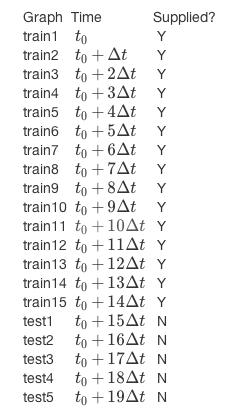
\includegraphics[scale=.5]{trainAndTestGraphs.png}
  \end{center}
\end{wrapfigure}

The domain of the data in this problem are the connections between
autonomous systems[2] in the Internet.  More specifically, the nodes in the
graph correspond to gateway routers for independent networks, and the directed
edges between them encode the network peering relationships with edge weight
indicating cost type of
transit over those links.

The training dataset consists of 15 graphs with anywhere from 46,603 to 49,520 directed edges each (so on the
order of ~750,000 edges total).  Each graph was collected at sequential time
points indicating operational direct connections and their cost types in the
network known at that point in time.  The format of each edge in the
training graph is \texttt{tail router AS Name | head router AS
  Name | cost type for use of the link} where the cost type is either 0 for ``free'' or 1
indicating that a fee is to be paid.  The number of unique node names in the
training dataset is 372,037 but part of the competition is to figure out
which of those "messy" names are duplicates.  A training edge may look like:

\texttt{{\small GOOGLE-CORPNET Google Ireland Limited | FACEBOOK-CORP - Facebook Inc | 1}}

The test dataset consists of 10,000 single or multi-edge paths for the (unobserved)
graphs at the next five time intervals.  A test path may look like:

\texttt{{\small REDWIRE - VoloNet Technologies, Inc | NCN-AS FOP Sergey Sergeevich | DKB | JMC-AS - JPMorgan Chase \& Co. | PIERCE-COUNTY - Pierce County}}

\subsection{Learning}

Although this competition could be performed using batch machine learning,
for the purposes of this project the problem will be reformulated as one for
online machine learning.  The edges in each training graph will be randomly
permuted and then fed incrementally to the learning algorithm, with all the
edges of graph 1 streamed prior to those of graph 2, etc...

Note that to meet the goals of this competition, two models are needed: (1)
a classification model for edge existence and (2) a classification model for
edge cost type.  Both will be learned incrementally as the edge data streams in
and will reuse features.

\textbf{Challenges}
\begin{itemize}
\item changing dimensionality of feature space: edges will come and go with time
\item temporality: edges will change costs with time
\item incomplete data: edges may be absent from the data but still exist
\item messy data: node names are mangled in the data and de-duping is needed
\end{itemize}

\section{Software and Algorithms}

\subsection{Data Cleaning}
Software was written to normalize and deduplicate the ``messy'' node names
found in the input data.  Techniques such as tf-idf were used to determine
which term(s) to remove from a multi-word node name to see if it
corresponded to a shorter word name.  This is the only batch process in the project; everything else is streaming.

\subsection{Features and Outcomes}

\textbf{Modeling Connections} A feature is created for each $(tail,head)$ pair and then hashed[3] into a
constrained dimensional space since we do not know the true dimensionality
of our input space.  

\textbf{Modeling Connectedness} A feature is created for the degree of each node
  involved in the edge  and then hashed[3] into a
constrained dimensional space since we do not know the true dimensionality
of our input space.  There are some nodes in
  the data which are very high degree and likely to be robust in terms of
  existence.  The value for this feature will be approximated rather than
  exact to adhere with our streaming data and its incomplete nature.  The feature value will be facilitated by the use of a
  bloom filter for each node observed encoding the set of nodes to which
  this node is connected.  The degree will be approximated by the
  number of bits set to true in the bloom filter.  

\textbf{Modeling Temporality} NEED ADVICE HERE

\subsubsection{Edge Cost Type Model}
Let $s$ and $t$ be two nodes in the graph at time $t$.  Then we have

$y_{cost\{u \rightarrow v\}}^{(t)} \in \{0,1\}$ 

where $1$ means that a fee must be paid for
traffic traversing the edge directly
between $s$ and $t$ and $0$ means that there is no fee.

$x_{cost\{u \rightarrow v\}}^{(t)} \in R^{d+h}$ 

is a column vector of length $n+m$
where 
\begin{itemize}
\item $n$ is the dimension of the space into which we've hashed our node names
\item $m$ is the dimension of the space into which we've hashed our directed
edge names
\end{itemize}

The vector which consists of the following features created from
edge $u \rightarrow v$ and the current epoch:
\begin{itemize}
\item The first $n$ values in $x$ are a Count-Min sketch of the degree of nodes in
  the graph.  For a particular $x$ this is sparse.  The only entries that will have values are the hashed entries for node $u$ and $v$.
\item The next $m$ values in $x$ are a Count-Min sketch of the number of
  times we have seen edges in the graph.  For a particular $x$ this is
  sparse.  The only entries that will have values is the hashed entry for
  edge $u \rightarrow v$ with value 1.
\end{itemize}

\subsubsection{Edge Existence Model}

Let $u$ and $v$ be two nodes in the graph at time $t$.  Then we have

$y_{exists\{u \rightarrow v\}}^{(t)} \in \{0,1\}$ 

where $1$ means that an edge exists directly
between $u$ and $v$, $0$ that the edge does not exist.  Note that in our
training data we only have outcomes where $y_{exists\{u \rightarrow v\}}^{(t)} = 1$.
Edges missing from the training data are assumed $y_{exists\{u \rightarrow v\}}^{(t)} = 0$.

$x_{exists\{u \rightarrow v\}}^{(t)} \in R^{d+h}$ 

is defined exactly the same as for the
edge cost model.

\subsection{Learning Algorithm}

Stochastic gradient descent will be used.  In addition to penalization via
regularization, weights will be boosted using the time interval $t$ so that more
recent data is emphasized.\footnote{I would greatly appreciate any
  suggestions as to how to better model recency of edges and also robustness
  of edges over time.  (e.g., a recent edge may have come and go repeatedly so it
  should be considered ``flaky''; a specific example may be routers in India
  where the power situation is sporadic.)}

\begin{displaymath}
w_i^{(t+1)} = w_i^{(t)} + epoch(t)*\tau*\eta \{- \lambda w_i^{(t)} + x_i^{(t)} [ y^t -  p(Y=1|x^{(t)},w^{(t)})] \}
\end{displaymath}
where $epoch(t) \in \{ 1,...,15 \}$ for each of our 15 training graphs.  In a more realistic situation, the epoch would be derived from the time at
which the edge information was received by the learner.

% \subsection{Prediction Pseudocode}

% \textsf{\small for each edge in the path, use the existence model to determine its probability of existence, multiply all the probabilities together}

% \textsf{\small for each edge in the path, use the cost model to determine its probable cost, sum all the costs together}

% \textsf{\small generate additional possible paths between tail and head (can keep graph generation simple at first and remove links in the test path to try shorter paths and/or replace intermediate nodes in the path with nodes of high degree)}

% \textsf{\small compute the existence probability and cost of each candiate path graph}

% \textsf{\small use decision theory to compare the test path with the candidate paths to determine the final prediction}

\section{Current Results}

\subsection{AS Name Cleaning}

Preprocessing was performed to compute a mapping of ``messy'' names to opaque
keys.  The software was able to reduce the number of unique node names from
372,037 to 44,015. For example the following key maps to 35 different unique node names
found in the data:

{\small \texttt{abccefkooopr abcefkoo|35|['FACEBOOK-CORP Inc - Facebook
    Inc', 'Facebook FACEBOOK-CORP - Facebook Inc', 'O-BEFKORACOPC - Facebook
    Inc', \\
... \\'FACEBOOK-CORP - Facebook Inc Inc', 'FACEBOOK-CORP FACEBOOK-CORP - Facebook Inc']}}

\subsection{Random Chance Prediction}

Kaggle leaderboard rankings are determined as follows: ``Your predictions
will be evaluated by the Area Under the ROC Curve (AUC) metric.  While the
ground-truth is binary, real-valued submissions are allowed. ``[1]  Included
is a screenshot of the ranking of a random chance prediction which will
serve at the baseline for this project.

  \begin{center}
    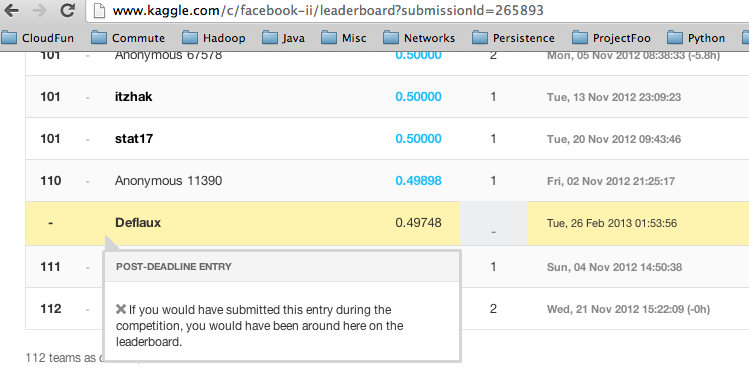
\includegraphics[scale=.4]{randomPredictions.png}
  \end{center}

\section{Discussion}

\section{Next Steps}

QUOTE TUBES HERE

penalize older history more heavily

~/rework/competitions/facebook2>find . -name *.java | xargs cat | wc -l
    2352
~/rework/competitions/facebook2>find . -name *.py | xargs cat | wc -l
     571
~/rework/competitions/facebook2>find . -name *.R | xargs cat | wc -l
      80
~/rework/competitions/facebook2>find src/main/ -name *.java | xargs cat | wc -l
    1130

\subsubsection*{References}

\small{
[1] \url{http://www.kaggle.com/c/facebook-ii/details/evaluation}

[2] \url{http://www.cisco.com/web/about/ac123/ac147/archived_issues/ipj_9-1/autonomous_system_numbers.html}

[3] Weinberger, Kilian, et al. {\it Feature hashing for large scale multitask learning." Proceedings of the 26th Annual International Conference on Machine Learning.} ACM, 2009.

[4] Nemirovski, Arkadi, et al. {\it Robust stochastic approximation approach to stochastic programming.} SIAM Journal on Optimization 19.4 (2009): 1574-1609.
}

\end{document}
